\documentclass[10pt,twocolumn,letterpaper]{article}
% the following 4 lines ar eadded
\makeatletter
 \def\@textbottom{\vskip \z@ \@plus 1pt}
 \let\@texttop\relax
\makeatother
%%%%%%

\usepackage{cvpr}
\usepackage{times}
\usepackage{epsfig}
\usepackage{graphicx}
\usepackage{amsmath}
\usepackage{amssymb}
\usepackage{epstopdf}
\usepackage{notoccite}

\DeclareGraphicsExtensions{.png,.pdf}

% Include other packages here, before hyperref.

% If you comment hyperref and then uncomment it, you should delete
% egpaper.aux before re-running latex.  (Or just hit 'q' on the first latex
% run, let it finish, and you should be clear).
\usepackage[pagebackref=true,breaklinks=true,letterpaper=true,colorlinks,bookmarks=false]{hyperref}

\cvprfinalcopy % *** Uncomment this line for the final submission

\def\cvprPaperID{cvpr.sty,v 1.3 2005/10/24 19:56:15 awf Exp} % *** Enter the CVPR Paper ID here
\def\httilde{\mbox{\tt\raisebox{-.5ex}{\symbol{126}}}}

% Pages are numbered in submission mode, and unnumbered in camera-ready
\ifcvprfinal\pagestyle{empty}\fi


\begin{document}

%%%%%%%%% TITLE
\title{Project Report: CS 7643 - Deep Learning Architectures for Material Selection and Structural Damage Detection}

\author{Hossein Daneshvar\\
Georgia Institute of Technology\\
North Avenue, Atlanta, GA 30332\\
{\tt\small hdaneshvar3@gatewch.edu}
% For a paper whose authors are all at the same institution,
% omit the following lines up until the closing ``}''.
% Additional authors and addresses can be added with ``\and'',
% just like the second author.
% To save space, use either the email address or home page, not both
\and
Mahshid Jafar Pour\\
Georgia Institute of Technology\\
{\tt\small mpour7@gatech.edu}
}

\maketitle
%\thispagestyle{empty}

%%%%%%%%% ABSTRACT
\begin{abstract}
   Climate change has led to increased incidences of hurricanes, extreme heat, flooding, and wildfires within our communities. These natural hazards in addition to earthquakes necessitate major changes to protect structures from these extreme loading events or mitigate their effects in the aftermath of natural disasters by moving towards more resilient structural solutions. While resilient structural design methodologies accounts for the probability of these extreme loading events, the need to balance the economics of the structure with the risk of structural failure under these extreme events, and possibly provide solutions for immediate recovery and occupancy of infrastructures in case of major events, is deemed crucial. Hence, rapid structural damage detection is an extremely useful tool to achieve resilient structures and communities. Owing to artificial intelligence (AI) and machine learning (ML) algorithms, in particular deep learning (DL) applications in image processing, structural health monitoring (SHM) in this context has grown extensively in recent years. In this project, we aim to contribute to this area of engineering by applying what we have learned in the CS-7643 DL course.  
\end{abstract}

%%%%%%%%% BODY TEXT
\section{Introduction/Background/Motivation}

In this project, the main objective is to combine the available DL methods learnt in the course with the structural health monitoring (SHM) application, specifically post-disaster structural damage recognition. The dataset created by the University of California Berkeley~\cite{Imagenet01} will be used as the main reference, called herein Structural ImageNet. The UC Berkeley research has applied only VGGNet architecture, while in this project, we are aiming to apply several other convolutional neural networks (CNN) architectures to study the Structural ImageNet tasks replacing the already used VGGNet, for instance, by ResNet~\cite{He01} or build our own network structure based on the insights obtained from the well-known available architechtures. Also, in the UC Berkeley research, instead of training deep CNN from scratch, deep Transfer Learning (TL) with VGG pretrained model is implemented, and feature extractor and fine-tuning as two TL strategies were introduced. With an increasing number of images, we are aiming to conduct the training process from scratch (i.e., without any pre-trained model), which is expected to have better performance. Complex recognition goals can be pursued, such as multiclass classification including the identification of many damage levels and multiple damage types for practical and broader use. To provide more useful information for real SHM applications, damage localization and quantification can be investigated additionally, in future.

A quick glance at the available literature in this area reveals that research on the intersection of structural health monitoring (SHM) and DL is quite limited. However, a quick glance at the available provides insight. Yu et. al~\cite{Yu01} proposed a CNN to identify and localize damages for the smart buildings instrumented with control devices. Their proposed network could automatically extract features from raw signals to meet the requirements of random objective functions. They used a high-dimension kernel in the first convolutional layer to reduce the noisy data such as AlexNet architecture. Also, several small-dimension kernels were utilized to characterize signal representations. Additionally, the ReLU function was used to mitigate overfitting. In the end, they developed a benchmark building equipped with smart isolators subjected to seismic excitation to assess the performance of their proposed model. Their proposed network demonstrated higher identification accuracy compared to other commonly used ML architecture~\cite{Yu01}. Rashid and Louis~\cite{Rashid01} used a recurrent neural networks (RNN) deep learning network to recognize construction equipment activities. For this task, they used data augmentation for training data and proposed a methodology to train and validate the long short-term memory (LSTM), with combined synthetic and real data. They tested their proposed model against so-called “traditionally used classification algorithms for construction equipment activity recognition” and observed enhanced performance~\cite{Rashid01}. Iannelli et al.~\cite{Iannelli01} proposed a Deep Neural Network, made of several neural network layers with different functions, in particular bi-directional LSTM layers, fully connected layers, and SoftMax, for structural damage detection for the study of a large system. The model was trained, validated, and tested by processing the time responses of the sensors using different damage scenarios such as the ones generated by the finite element codes. Their proposed model demonstrated good performance and accuracy~\cite{Iannelli01}.

Structural Health Monitoring (SHM) usually refers to engineering assessment and evaluation that study the structural integrity of structural components which are usually statics while in mechanical systems, with moving parts and assemblies, the process is called Condition Monitoring (CM) or Condition Health Monitoring (CHM) instead of SHM. In terms of the procedure employed, SHM or CHM systems are similar, which include the acquisition of structural response data over time and processing of the obtained dataset in order to identify features that contain information about possible or potential damage initiation and propagation~\cite{Seventekidis01}. In addition to the literature in the realm of SHM, publications in CHM area could be useful as well. For instance, Zhao et al.~\cite{Zhao01} performed a systematic literature review of deep learning-based machine health monitoring systems (MHMS), which the results found applicable to SHM as well due to the inherent similarities of mechanical and structural systems, as discussed. They categorized the DL-based MHMS into four classes of architecture i.e., auto-encoder models, restricted Boltzmann machines models, CNN, and RNN. During their investigations, they found that the satisfactory performance of employed DL architecture highly depends on the quantity and quality of datasets being used. While they called the deep neural networks as “black boxes” models, they hoped advances in data visualization may provide insights into some of the computation mechanisms used to solve structural health monitoring problems. They advocate the use of Transferred Deep Learning due to the lack of data in most MHMS areas. 
\\
Applications of SHM and CHM methods can span over a large group of structures such as bridges~\cite{Tome01} , ~\cite{Wickramasinghe01},~\cite{Yapar01} ,~\cite{Dohler01}, wind generators ~\cite{Garcia01}, ~\cite{Tcherniak01} or aircrafts ~\cite{Elasha01}, ~\cite{Ksica01}; however the application of DL in the modern SHM is a new topic which has gained attention over the last few years~\cite{Seventekidis01}, which is the topic of this research as well.

In SHM, there is a need to balance the economics of the structure design with the risk of structural failure under extreme events, and possibly provide solutions for immediate recovery and occupancy of infrastructures in case of major events.  Knowing the type of material we are dealing with and the type of damage is always the first step. Therefore, fast structural damage detection is an extremely useful tool to achieve resilient structures and communities. 

%-------------------------------------------------------------------------
\section{Dataset}
The abbreviated employed “Structural ImageNet” is a large-scale open-sourced structural image database called the “PEER (Pacific Earthquake Engineering Research Center) Hub ImageNet ($\Phi$-Net)”~\cite{Imagenet01}. As of November 2019, this $\Phi$-Net dataset contains 36,413 images with multiple attributes for the following baseline recognition tasks: scene-level classification, structural component type identification, crack existence check, and damage-level detection. According to the UC researchers at Berkeley, there is no other open-sourced structural image dataset with multi-attribute labels and this volume of images in the vision-based SHM area. It is believed that this image dataset and its corresponding detection tasks and framework will provide the necessary benchmark for future studies of DL in vision-based SHM.
Here is the link to the dataset: 
https://apps.peer.berkeley.edu/phi-net/ 
\\
The dataset has been divided into eight subsets of scene level, damage state, spalling condition, material type, collapse mode, component type, damage level, and damage type~\cite{Gao01} \cite{Gao02} \cite{Gao03}. A sample of damage type classes are shown in the Figures 1 to 2. Our work is focused on task 4 (material type) and 8 (damage type). 
Task 4 is considered easy and has two classes while task 8 is considered difficult and has 4 classes, all images have size $224\times224\times3$. The details of each dataset are summarized in Table 1.

\begin{table*}
\begin{center}
\begin{tabular}{|c|c|c|c|c|c|c|}
\hline
Dataset & Train Size & Test Size & Class 0 ($\%$ in train) &  Class 1 ($\%$ in train) & Class 2  ($\%$ in train) & Class 3  ($\%$ in train) \\
\hline\hline
Task 4 & 8321 &  979 & Other Material (78.27$\%$) & Steel (21.73$\%$) & NA & NA \\
\hline
Task 8 & 4093 & 492 & Combination  (29.15$\%$)  & Undamaged (11.63$\%$) & Flexural (39.04$\%$) & Shear (20.18$\%$) \\
\hline
\end{tabular}
\end{center}
\caption{Data Statistics.}
\label{tab:dataset}
\end{table*}


\begin{figure}[t]
\begin{center}
%\fbox{\rule{0pt}{2in} \rule{0.9\linewidth}{0pt}}
   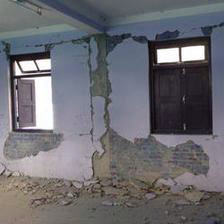
\includegraphics[width=0.8\linewidth]{data0.png}
\end{center}
   \caption{Sample of data for damage type detection (four classes: undamaged, flexural damage, shear damage, combined damage)~\cite{Imagenet01}}
\label{fig:long1}
%\label{fig:onecol}
\end{figure}

%\begin{figure}[t]
%\begin{center}
%%\fbox{\rule{0pt}{2in} \rule{0.9\linewidth}{0pt}}
%   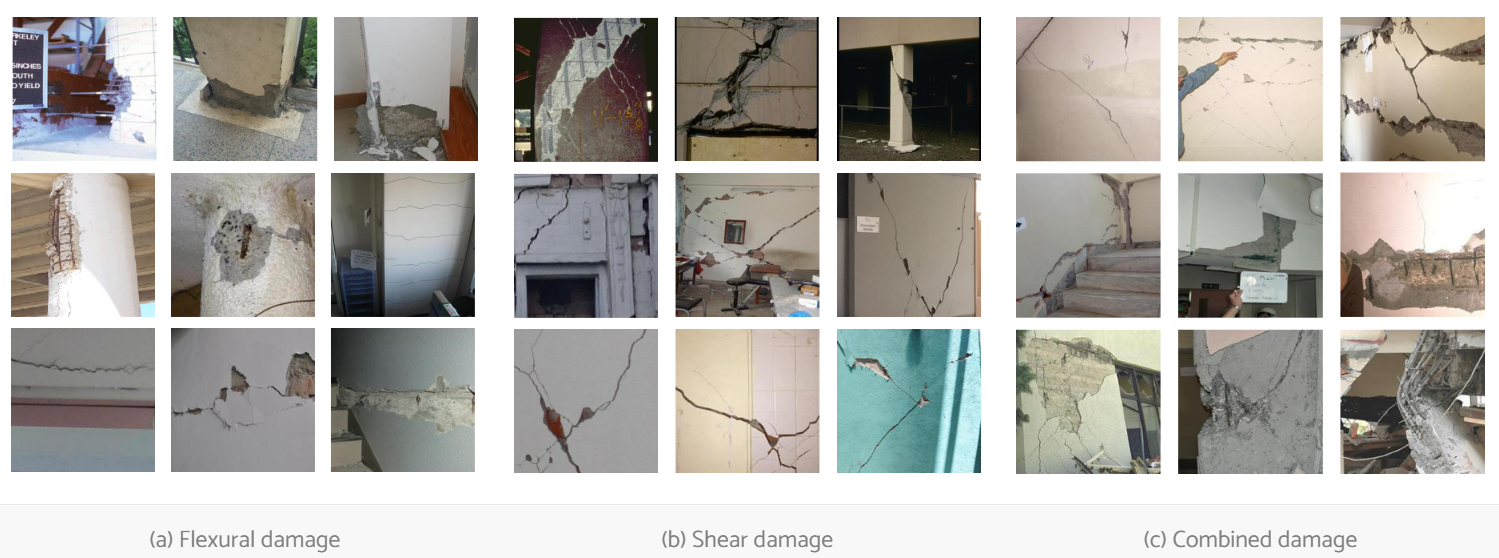
\includegraphics[width=1.8\linewidth]{damageType}
%\end{center}
%   \caption{Types of damage~\cite{Imagenet01}}
%\label{fig:long}
%\label{fig:onecol}
%\end{figure}
%-------------------------------------------------------------------------
%------------------------------------------------------------------------
\section{Approach}
In essence, we used deep CNN to classify images. We tried different architectures such as VGGNet, and ResNet and compared the obtained results. After gaining experience by applying available well-known architecture and evaluating their performance, we build our own architecture and applied it to the dataset. Considering the small size of the dataset, we could not train the model effectively. Although the results look promising when data augmentation and transfer learning ~\cite{ref03} are applied.  
\subsection{Data Pre-Processing}
One of the current disadvantages of image datasets in the realm of structural health monitoring (SHM) is the limitation of data size, in terms of the number of pictures. This lack of a sufficient number of pictures may cause several problems such as overfitting i.e. when the CNN learns a highly variant function~\cite{Shorten01}. To avoid such undesired performance, data augmentation is employed, which is a suite of techniques that enhance the size and quality of training datasets e.g., geometric transformations, color space transformations, kernel filters, mixing images, random erasing, etc. Data augmentation is the novel contribution in this research as the researchers at Berekley have only applied one form of image augmentation called fancy-PCA. Figure 2 (a) shows a random image of a wall with orthogonal cracks, while Figures 2 (b), (c), and (d) show the same images after random rotation, blurring, and flipping operations. It is noted that image cropping, while largely popular in other applications, is deliberately avoided herein to prevent removing the damage from the image.
Since the material type data set is imbalanced, i.e., one class of data is larger than the other one, over-sampling of the smaller class has been performed to achieve more balance. Additionally, after the data augmentation, data normalization is performed to achieve a more stable model training.  

\begin{figure}[t]
\begin{center}
   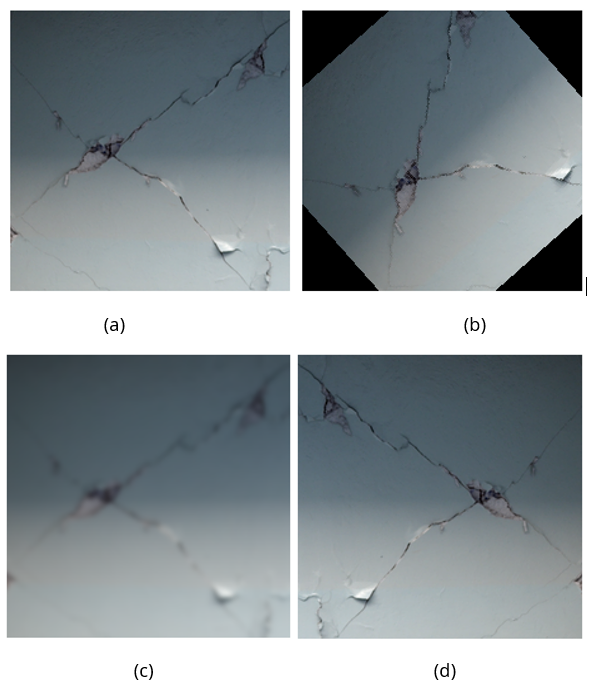
\includegraphics[width=0.8\linewidth]{dataAug}
\end{center}
   \caption{Data Augmentation: (a) original image (b) random rotation (c) blurring (d) flipping ~\cite{Imagenet01}}
\label{fig:long2}
\end{figure}

\subsection{Challanges}
There are several challenges involved in this project. Due to the size of the data set, training the whole model was not successful despite trying different structures, and we found that transfer learning is a must. In addition to the limited size of the dataset, we anticipated issues with imbalanced data: for Task 4, class 1 is 21.73$\%$ of the train dataset, and for task 8 class 1 is 11.6$\%$ of train dataset (see Table 1).  We are tackling this challange by oversampling small class in data augmentation step. 

\subsection{Modeling}
We started with Task 4 (material type identification), which is considered easy. We built a customized architucture with 5 convolutional layers, maxpooling, average pooling layers with ReLu as the activation function and 2 dropouts and 3 fully-connected layers. However, trainig the model was not successful due to limited number of images compared to the number of parameters the model has to learn. We tried to lower the number of layers and it did not help. During training, a reduction in train loss was observed, but there was no improvement in the class/overall accuracy and the model predicted all the images as class 0 (the dominant class). However, when we used transfer learning with VGG-16 and froze all layers except the last layer, a significant improvement was observed. For comparison, we tried other structures such as VGG-16-BN and ResNet50, both predicted well.

The imbalanced dataset was addressed by oversampling the smaller class in data augmentation and reducing batch size. We tried differnt types of losses: Cross-entropy loss (CE), focal loss and negative log-likelihood loss (NLLL), the last two are known to perfom better for imbalanced datsets. However, focal loss did not improve the results. Overall, NLLL and CE results are very close, especially for task 4, but NLLL gives slightly better accuracy. 

Once we found the right loss, transfer learning and the architechtures that perform well, we moved to the more difficult task (task 8 damage type identification) which has even less data. For both tasks, ResNet50 ended up to be the best network structure. Hyper-parameter tuning of the two tasks are implemented separately.

All the abovementioned work was performed using Pytorch versions 1.12.1 and 1.13.0 on GPU.  


%-------------------------------------------------------------------------
\section{Experiments and Results}
The main measure for performance evaluation of the employed models was the confusion matrix, and assuring that the class accuracy and overall accuracy are increasing. Figures 3 and 4 show the class accuracy with epochs for Task 4 and 8 respectively. 
A manual grid search was used to achieve an optimum hyper-parameters set. It was observed that the learning rate in the order of 1e-4 produces the most accurate results. SGD optimizer with momentum and regularization was selected since Adam optimizer is well known to perform worse than SGD for image classification tasks~\cite{Gupta01}. 

The batch size was found to be the most important hyper-parameter that affects training. On task 4, with larger batch sizes, the model predicts only one class. As the batch size reduces the model performance improves significantly. Using a batch size of 8 the model learns quickly, but it is observed that most of the learning happened in the first epoch, with minor improvements afterward. While a model with a batch size of 16, learns in higher epochs, its performance is lower, compared to a model with a batch size of 8 (See Figure 3). It was counter-intuitive at first, since a bigger batch size is more representative of the datset, but we realized with smaller batch size we are updating the learnable parameters more. Eventually, batch sizes of 8 and 16 were selected for tasks 4 and 8 respectively, as they yield the best model performance in terms of accuracy.

Additionally, regularization of 1e-3 and momentum of 0.9 were found to provide the best performance in terms of accuracy. Tables 2 and 3 summarize the results of different structures while table 4 summerizes the finalized hyper-parameters implemented in the best models. ResNet50 has the highest accuracy for both datasets. With ResNet50 architecture, our results could beat the accuracy achieved by~\cite{Gao01}, they had overall accuracy of 63.05$\%$ for task 8 while our accuracy is 67.48$\%$ . They however, have higher accuracy for the smaller class. Gao et al.~\cite{Gao01} mentioned one of the contributors to achieving high accuracy was applying fancy-PCA as part of image augmentation, which we did not get a chance to try. 

 \begin{figure}[t]
\begin{center}
   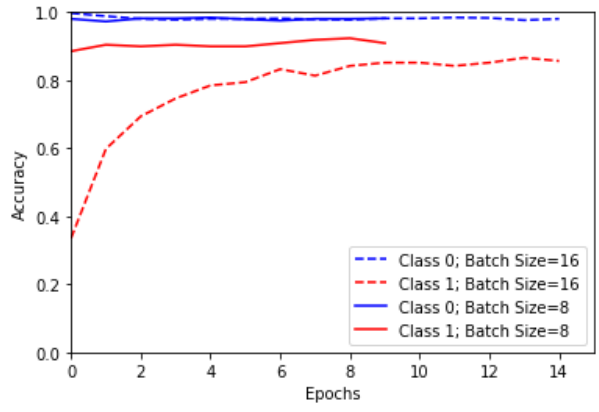
\includegraphics[width=0.8\linewidth]{task4Curves}
\end{center}
   \caption{Task 4 Class accuracy curves with epochs/Effect of batch size}
\label{fig:long3}
\end{figure}

\begin{figure}[t]
\begin{center}
   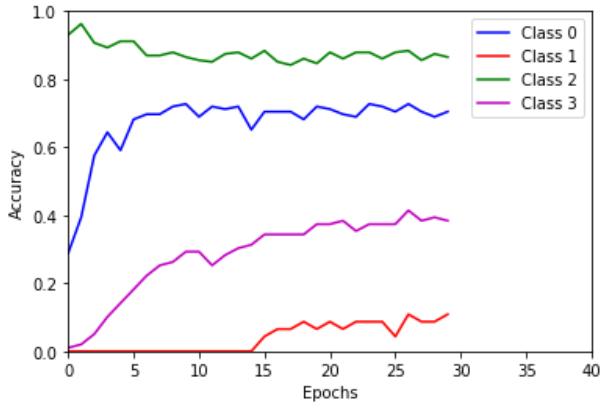
\includegraphics[width=0.8\linewidth]{task8Curves}
\end{center}
   \caption{Task 8 Class accuracy curves with epochs}
\label{fig:long4}
\end{figure}

The model predictions on the test dataset (unseen data) are reasonable and not very different from the accuracy of the training set; therefore, there is no overfit of the model. The final confusion matrix of the best model employed is shown in Figure 5 and 6 for tasks 4 and 8 respectively.

\begin{figure}[t]
\begin{center}
   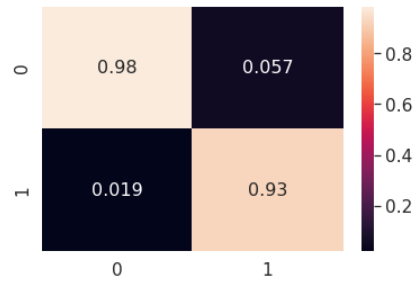
\includegraphics[width=0.8\linewidth]{task4cm}
\end{center}
   \caption{Task 4 confusion matrix}
\label{fig:long5}
\end{figure}

\begin{figure}[t]
\begin{center}
   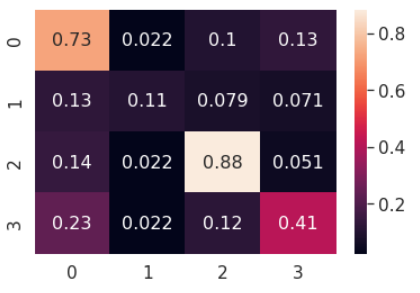
\includegraphics[width=0.8\linewidth]{task8cm}
\end{center}
   \caption{Task 8 confusion matrix}
\label{fig:long6}
\end{figure}

\begin{table*}
\begin{center}
\begin{tabular}{|c|c|c|c|}
\hline
Model & Class 0 Accuracy & Class 1 Accuracy  & Overall Accuracy \\
\hline\hline
Customized & 1.0 &  0.0 & 0.7865 \\
\hline
VGG16 & 0.9779 & 0.9330 & 0.966 \\
\hline
VGG16-BN & 0.9766 & 0.8900 & 0.9551 \\
\hline
ResNet50  & 0.9884 & 0.9282 & 0.9724\\
\hline
\end{tabular}
\end{center}
\caption{Comparison of different structures on Task 4.}
\label{tab:Task4Result}
\end{table*}

\begin{table*}
\begin{center}
\begin{tabular}{|c|c|c|c|c|c|}
\hline
Model & Class 0 Accuracy & Class 1 Accuracy & Class 2 Accuracy &  Class 3 Accuracy & Overall Accuracy \\
\hline\hline
Customized &  0.0 & 0.0 & 1.0 & 0.0 & 0.4370 \\
\hline
VGG16 & 0.6212 & 0.1739 & 0.8465 & 0.4040 & 0.6341 \\
\hline
VGG16-BN & 0.6364 & 0.1304 & 0.8372 & 0.3737 & 0.6240 \\
\hline
ResNet50 & 0.7273 & 0.1087 & 0.8837 & 0.4141 & 0.6748 \\
\hline
\end{tabular}
\end{center}
\caption{Comparison of different structures on Task 8.}
\label{tab:Task8Result}
\end{table*}

\begin{table*}
\begin{center}
\begin{tabular}{|c|c|c|}
\hline
 & Task 4 & Task 8 \\
\hline
Best Parameters & ResNet50 &  ResNet50 \\
\hline\hline
Batch Size & 8 & 16 \\
\hline
Epochs & 10 & 30 \\
\hline
Learning Rate  & 1e-4 & 1e-4 \\
\hline
Regularization  & 1e-3 & 1e-3 \\
\hline
Momentum  & 0.9 & 0.9 \\
\hline
Loss  & CE/NLLL & NLLL \\
\hline
\end{tabular}
\end{center}
\caption{Best model configuration.}
\label{tab:hyperparam}
\end{table*}

%-------------------------------------------------------------------------
\section{Conclusions}
One of the main observations was that training a model from scratch for such small data set was very ambitious; however, using transfer learning, significant improvements have been observed in the results. We tried different architectures and as expected ResNet50 with transfer learning was able to improve model accuracy compared to other architectures. The results outperformed the accuracy achieved by~\cite{Gao01}, they had overall accuracy of 63.05$\%$ for task 8 while our accuracy is 67.48$\%$. Applying other methods, within the data augmentation domain, to expand the dataset will improve the results which are determined to do so after this course completion, as a future endeavor.   

%-------------------------------------------------------------------------
\section{Other Sections}
\subsection {Resources}
We used parts of the Assignment 2 code with some modifications for it to be suitable for this dataset.

The focal loss was attempted from this repository ~\cite{repo01}, although it was not used as the final loss used in the models. 

The following resources are used for transfer learning: ~\cite{ref01}, ~\cite{ref02}, ~\cite{ref03}.


\section{Work Division}
%-------------------------------------------------------------------------
\begin{table*}
\begin{center}
\begin{tabular}{|l|p{4cm}|p{4cm}|}
\hline
Student Name & Contributed Aspects & Details \\
\hline\hline
Hossein Daneshvar &  Literature review, EDA, Data preprocessing, Hyperparameter tuning, Transfer learning, Report  &  Topic and dataset search, literature review, preliminary EDA, image augmentation, hyper-parameter tuning, accuracy plots, transfer learning, report writing, final report review \\
\hline
Mahshid Jafar Pour &  EDA, Data preprocessing, customized model, code for CNN training, Hyperparameter tuning, Report & EDA and visulaization of data, data normalization, main code for training, customized model architecture, confusion matrix, hyper-parameter tuning, report writing, LaTeX format, final report review\\
\hline
\end{tabular}
\end{center}
\caption{Contributions of team members.}
\label{tab:contributions}
\end{table*}

%-------------------------------------------------------------------------


{\small
\bibliographystyle{ieee_fullname}
\bibliography{egbib}
}

\end{document}
